\chapter{Basics and essential concepts of (Deep)ProbLog} \label{problog_deepproblog_essentials}
In this appendix, we will give a bird's-eye view of ProbLog and its extension DeepProbLog. Basic knowledge of Prolog (and logic programming) is assumed. We advise consulting a work like \cite{learnprolognow} to readers unfamiliar with it. ProbLog has excellent in-depth documentation by \cite{problog_documentation} that provides all information about it and its many features beyond what is required to understand this paper and will be covered here.

This content on ProbLog was borrowed and paraphrased from the 2022 lecture by Dr. Luc De Raedt on it within the KU Leuven course of Uncertainty in Artificial Intelligence organized by Dr. Tinne De Laet.

\section{ProbLog concepts}
ProbLog can be seen as a Prolog extension allowing facts and clauses to be true or qualified stochastically by either a known or to be inferred probability. In other words, ProbLog is an extension of Prolog's semantics such that ProbLog programs can represent Bayesian belief network models as well as the traditional boolean network models that can be represented by Prolog. ProbLog allows answering not only logical but also probabilistic queries. It's thus an intriguing base for the field of StarAI, or \textbf{Sta}tistical \textbf{R}elational \textbf{A}rtificial \textbf{I}ntelligence, similar to how neural networks are an interesting base for the fields of computer vision and natural language processing. We can refer to ProbLog KBs as probabilistic logic programs and to the clauses in them as probabilistic clausal laws.
Prolog inference on the one hand is based on the renowned unification algorithm \cite{how_prolog_works}. ProbLog inference on the other hand is based on weighted model counting/weighted \#SAT solving. The following steps are carried out by ProbLog to answer a query:
\begin{enumerate}
  \item Grounding the KB with respect to the variable values given in the query
  \item Converting the ground KB into a propositional logic formula
  \item Conpiling that formula to an arithmetic circuit
  \item Evaluating the arithmetic circuit
\end{enumerate}

\section{Basic use, structure and syntax of ProbLog KBs}
ProbLog is distributed as a Python (PyPI) package. When installed using pip, it will be available on the system as a command line program and as a set of modules for use in Python scripts. ProbLog KBs can be stored in plain-text files with an extension such as \texttt{.pl}. ProbLog KBs containing queries and/or evidence can then be processed by running a command like \lstinline[columns=fixed]{problog <path/to/the/knowledge_base>.pl} in the terminal. More detailed and concrete installation instructions for specific platforms and use cases are available online.\footnote{\href{https://problog.readthedocs.io/en/latest/install.html}{ProbLog installation instructions}}

The syntax of ProbLog is largely analogous to Prolog's. The main novelty is the \texttt{::} operator, which is used to specify the (un)known probability of a clause or fact. A fact with a known probability of 0.1 would, for example, be written as:
\begin{lstlisting}[language=Prolog]
0.1 :: fact.
\end{lstlisting}
A clause with the same known probability would be written in the KB as:
\begin{lstlisting}[language=Prolog]
0.1 :: head :- body.
\end{lstlisting}
ProbLog can also learn unknown probabilities in the Learning From Interpretations (LFI) mode. In this mode the unknown probability is indicated using the \texttt{t}-functor. For example, to declare a fact with an unknown probability that ProbLog has to learn in LFI mode, one would write:
\begin{lstlisting}[language=Prolog]
t(_) :- fact.
\end{lstlisting}
The argument of the \texttt{t}-functor can be either a probability that is used as the initial value during learning or \texttt{\_} if a random initial probability value should be chosen during LFI. LFI learns the probabilities based on evidence given in another KB using the built-in \texttt{evidence}-functor. To run in LFI mode one would for example run the command \lstinline[columns=fixed]{problog lfi <model> <evidence> -O <output model>}.

An auxiliary ProbLog concept is the annotated disjunction (AD), which is used to create probability distributions for facts and clause heads. For example, the throw of a die can be modelled as follows:
\begin{lstlisting}[language=Prolog]
1/6::die(D, 1); 1/6::die(D, 2); 1/6::die(D, 3);
1/6::die(D, 4); 1/6::die(D, 5); 1/6::die(D, 6).
\end{lstlisting}
Should probabilities not add up to one, an implicit null choice is created in which none of the facts in the AD are true with the remaining probability.

We will show the basic structure, syntax and interpretation of a complete ProbLog KB by means of modelling and querying the simple yet well-known burglar-alarm Bayesian belief network and a more complex problem of predicting student grades. Figure \ref{fig:burglar_alarm_network} shows the Bayesian belief network model of the burglar-alarm case while listing \ref{lst:burglar_alarm_problog} shows the corresponding ProbLog model:
\begin{figure}
  \centering
  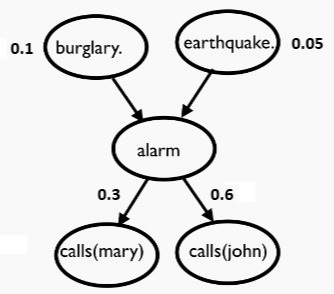
\includegraphics[width=0.6\linewidth]{images/burglar_alarm_network.jpg}
  \caption[The canon burglar-alarm Bayesian belief network]{The canon burglar-alarm Bayesian belief network}
  \label{fig:burglar_alarm_network}
  \source{\textcopyright 2022 Dr. Luc De Raedt}
\end{figure}

\begin{lstlisting}[language=Prolog, caption={burglar\_alarm.pl, the burglar alarm Bayesian belief network}, numbers=left, label={lst:burglar_alarm_problog}, captionpos=b]
0.1 :: burglary.
0.05 :: earthquake.

alarm :- burglary.
alarm :- earthquake.

0.3 :: hears_alarm(mary).
0.6 :: hours_alarm(john).

calls(mary) :- alarm, hears_alarm(mary).
calls(john) :- alarm, hears_alarm(john).
\end{lstlisting}
Like in the original belief network, this logic program represents that
\begin{itemize}
  \item a burglary or an earthquake have a certain chance of happening at a given time
  \item the occurrence of a burglary or an earthquake always triggers the alarm
  \item John and Mary have a chance of hearing the alarm if it goes off
  \item John and mary both always call the police if they hear the alarm going off
\end{itemize} 

This program contains four probabilistic facts: 
\begin{itemize}
  \item \texttt{burglary}: line 1, 10\% chance of being true,
  \item \texttt{earthquake}: line 2, 5\% chance of being true,
  \item \texttt{hears\_alarm(mary)}: line 7, 30\% change of being true,
  \item \texttt{hears\_alarm(john)}: line 8, 60\% change of being true
\end{itemize}

Next consider listing \ref{lst:student_grading_problog} which models a student grade prediction ontology. Consider the following variables and predicates:
\begin{itemize}
  \item S, C: variables representing students and courses respectively
  \item intelligent(S): probabilistic fact indicating whether S is an intelligent student
  \item grade(S, C, G): probabilistic fact indicating that student S achieved grade G for course C
  \item difficult(C): probabilistic fact indicating that course C is difficult
\end{itemize}
Now, listing \ref{lst:student_grading_problog} models that a given student has a 40\% change of being intelligent and a course C has a 50\% chance of being difficult using the probabilistic clauses on line 4 and 5. Then, depending on the intelligence of students and the difficulty of courses probability distributions over students' grades conditioned on courses are defined on line 8, 12 and 17 of listing \ref{lst:student_grading_problog} using ADs on clause heads. Finally, the concepts of unsatisfactory and excellent students are defined in listing \ref{lst:student_grading_problog} based on the preceding probabilistic clauses and facts.
\begin{lstlisting}[language=Prolog, caption={student\_grading.pl, the student grading problem}, numbers=left, label={lst:student_grading_problog}, captionpos=b]
student(john). student(anna). student(bob).
course(ai).    course(ml).    course(cs).
  
0.4 :: intelligent(S) :- student(S).
0.5 :: difficult(C) :- course(C).
  
grade(S, C, a) :- intelligent(S), not difficult(C).
0.3 :: grade(S, C, a);
  0.5 :: grade(S, C, b);
  0.2 :: grade(S, C, c) :-
    intelligent(S), difficult(C).
0.1 :: grade(S, C, b);
  0.2 :: grade(S, C, c);
  0.2 :: grade(S, C, f) :-
    student(S), course(C),
    not intelligent(S), not difficult(C).
0.3 :: grade(S, C, c); 0.2 :: grade(S, C, f) :-
  not intelligent(S), difficult(C).
  
unsatisfactory(S) :- student(S), grade(S, C, f).
excellent(S) :-
  student(S),
  not( grade(S, C1, G), below(G, a) ),
  grade(S, C2, a).
\end{lstlisting}
In ProbLog, queries and evidence can be included in the KB (for example to turn the KB into a stand-alone executable program). This is done by adding \texttt{query} and \texttt{evidence} facts having the terms of the query or the evidence as their argument. To include the query \texttt{calls(mary)} in the burglar-alarm example (to get the probability with which Mary calls the police) given the evidence that an earthquake occurred, we would add the following lines to the end of listing \ref{lst:burglar_alarm_problog}:
\begin{lstlisting}[language=Prolog]
evidence(earthquake).
query(calls(mary)).
\end{lstlisting}

\section{Managing and querying ProbLog KBs from Python}
When working with Python in an environment where the \texttt{problog} PyPI package is installed, we can process ProbLog KBs using all of its inference engines from our modules. This allows ProbLog KB processing to be embedded in a vast variety of systems and applications.

We can take varying degrees of control while using ProbLog in Python. Listing \ref{lst:basic_python_burglar_alarm} shows a high level program to get the results of KB queries:
\begin{lstlisting}[language=Python, caption={basic\_burglar\_alarm.py, high level burglar-alarm model querying in Python}, numbers=left, label={lst:basic_python_burglar_alarm}, captionpos=b]
from problog import get_evaluatable
from problog.core import ProbLog
from problog.program import PrologFile
from problog.sdd_formula import SDD

if __name__ == "__main__":
  burglar_alarm_KB = PrologFile("burglar_alarm.pl")
  burglar_alarm_query_results = get_evaluatable() \
    .create_from(burglar_alarm_KB) \
    .evaluate()
  for query, result in burglar_alarm_query_results.items():
    print(f"{query}: - {result}")    
\end{lstlisting}
Taking finer-graind control, however, is also possible, as Listing \ref{lst:low_level_python_burglar_alarm} shows.
\begin{lstlisting}[language=Python, caption={low\_level\_burglar\_alarm.py, low level burglar-alarm model querying in Python}, numbers=left, label={lst:low_level_python_burglar_alarm}, captionpos=b]
from problog import get_evaluatable
from problog.engine import DefaultEngine
from problog.logic import Constant, Term
from problog.program import PrologFile

if __name__ == "__main__":
  burglar_alarm_KB = PrologFile("burglar_alarm.pl")
  engine = DefaultEngine()
  prepared = engine.prepare(burglar_alarm_KB)
  query1 = Term('calls', Term("mary"))
  grounded = engine.ground_all(prepared, queries=[query1])
  compiled = get_evaluatable().create_from(grounded)
  results = compiled.evaluate()
\end{lstlisting}

\section{DeepProbLog concepts}
DeepProbLog extends ProbLog with neural predicates, which map inputs to outputs based on an underlying neural network (NN). Neural predicates can be seen as a syntax to generate facts at inference time that connect inputs to outputs using a NN. In fact, no changes in the probabilistic host language are inherently needed: in principle DeepProbLog could be implemented on top of any of them.
NN classifiers often output real numbers called logits for each class. Usually, the higher some class's logit is in comparison to the others, the more certain it is that the input sample belongs to this class. Thus, if the NN's outputs are then normalized they can be interpreted as a probability distribution over the classes. DeepProbLog's neural predicates can leverage this to generate probabilistic facts using the NN too. These predicates can accordingly map inputs to output probability distributions. This is, in fact, the most important use of neural predicates in practice.

One of the most important aspects of DeepProbLog to understand is how the NNs that make up a DeepProbLog model are trained. In traditional NN training, a dataset is a mapping of a preferably large number of example inputs and the corresponding desired NN outputs, called targets. In the DeepProbLog context, no datasets for individual NNs are needed at all. A dataset of ground queries that must hold is given. Individual NN weights are adjusted during training such that the model as a whole reproduces the given query truths as well as possible.

\section{Syntax of DeepProbLog KBs}
In DeepProbLog, the special functor \texttt{nn} is used to declare a neural predicate. The \texttt{nn} functor has an arity of four, with three arguments being optional:
\begin{enumerate}
  \item The name of the underlying NN (which is used to couple the neural predicate to the NN)
  \item The list of input variables
  \item The output variable
  \item The different values the output variable can take, i.e. the different possible classes. (It is optional but is used most of the time. An example of when it is not used is when declaring neural predicates for encoder NNs.)
\end{enumerate}
The \texttt{nn} functor is always used on the left-hand side of the \texttt{::} operator. On the right hand side of the \texttt{::} operator, the predicate is defined as a fact or clause head using the input and ouput variables specified as the second and third argument of the \texttt{nn} functor.
Consider the following neural predicate definition:
\begin{lstlisting}[language=Prolog]
nn(mnist_net, [X], Y, [0 ... 9] ) :: digit(X, Y).
\end{lstlisting}
This neural predicate defines that a NN called \texttt{mnist\_net} with one input, \texttt{X} (here a tensor representing an image), and output \texttt{Y} which can be a number from 0 to 9 is represented in the KB by a clause named \texttt{digit} that takes in \texttt{X} and outputs \texttt{Y}. This neural predicate will get instantiated at inference time into a neural annotated disjunction (nAD), or set of probabilistic facts, such as the following:
\begin{lstlisting}[language=Prolog]
0.04 :: digit(<first_image>, 0); 0.35 :: digit(<first_image>, 1); ... ;
0.53 :: digit(<first_image>, 7); ... ; 0.014 :: digit(<first_image>, 9).
\end{lstlisting}

\section{Managing and querying DeepProbLog KBs from Python}
\label{managing_querying_DeepProbLog_from_python}
It is first and foremost important to understand that DeepProbLog KBs need to be processed using Python. Python acts as the bridge between the DeepProbLog probabilistic logic program and the NNs included in the DeepProbLog probabilistic logic progam's neural predicates. DeepProbLog itself only comes as a Python package because of this. At the time of writing, DeepProbLog was not published as a PyPI package yet. The DeepProbLog codebase with additions relevant to this paper can be found in this paper's \href{https://github.com/Joshua-Schroijen/deepproblog/tree/master/src/deepproblog/examples}{accompanying GitHub repository}. In the root of this repository a file named \texttt{EXTRA\_USAGE\_INSTRUCTIONS.md} can be found containing detailed installation instructions. In the folder \texttt{src/deepproblog/examples} several examples of Python scripts utilising DeepProbLog for various applications can be found. 

There are three essential components to a DeepProbLog application:
\begin{enumerate}
  \item A complete KB/\texttt{.pl} file, which can have neural predicates
  \item Proper neural network topologies for the base NNs of aforementioned neural predicates
  \item Datasets of queries on the KB from which unknown KB probabilities/parameters and NN weights can be learned. To include complex data objects, queries can contain terms referencing arbitrary tensors from a user-defined tensor source.
\end{enumerate}
These components are brought together by a driving Python script. The PyTorch library is used to provide NNs. These scripts will always follow roughly the following flow:
\begin{enumerate}
  \item Load and create dataset objects (of (sub)type \texttt{deepproblog.dataset.Dataset}).
  \item Create data loader objects based on the dataset objects (of (sub)type \\\texttt{deepproblog.dataset.DataLoader})
  \item Create PyTorch NN objects
  \item Create DeepProbLog network objects (type \texttt{deepproblog.network.Network}) based on the PyTorch NNs
  \item Construct a DeepProbLog model object (type \texttt{deepproblog.model.Model}) based on the KB file and the DeepProbLog Network objects
  \item Create an engine object and add it to the model. An approximate (class \texttt{deepproblog.engines.ApproximateEngine}) and exact (class \\\texttt{deepproblog.engines.ExactEngine}) inference engine are provided in the standard DeepProbLog distribution. Both engines have cases in which they are or are not appropriate.
  \item Couple tensor source objects to the model using its \texttt{add\_tensor\_source} method
  \item Use the \texttt{deepproblog.train.train\_model} function to train the DeepProbLog model (which means optimizing the unknown model probabilities/parameters and the model's NNs' weights for model cross-entropy loss)
\end{enumerate}

Let us illustrate the preceding concepts by looking at the single-digit MNIST addition example application which can be found in the file \\\texttt{src/deepproblog/examples/MNIST/addition.py}. The comments in the listing indicate which of the previous steps is being carried out.
\begin{lstlisting}[language=Python, caption={src/deepproblog/examples/MNIST/basic\_addition.py, the basic MNIST single-digit addition example}, numbers=left, label={lst:MNIST_addition_source_code}, captionpos=b]
import torch
from deepproblog.dataset import DataLoader
from deepproblog.engines import ApproximateEngine
from deepproblog.evaluate import get_confusion_matrix
from deepproblog.heuristics import geometric_mean
from deepproblog.model import Model
from deepproblog.network import Network
from deepproblog.train import train_model
from deepproblog.examples.MNIST.data import MNISTOperator, MNIST_train, MNIST_test
from deepproblog.examples.MNIST.network import MNIST_Net
  
if __name__ == "__main__":
  # General DeepProbLog flow - step 1
  # Load and create dataset objects (of (sub)type deepproblog.dataset.Dataset)
  train_dataset = MNISTOperator(
    dataset_name = "train",
    function_name = "addition",
    operator = sum,
    size = 1,
    arity = 2
  )
  test\_dataset = MNISTOperator(
    dataset_name = "test",
    function_name = "addition",
    operator = sum,
    size = 1,
    arity = 2
  )
  
  # General DeepProbLog flow - step 2
  # Create data loader objects based on the dataset objects (of (sub)type deepproblog.dataset.DataLoader)
  batch_size = 2
  train_dataloader = DataLoader(train_dataset, batch_size, False)
  
  # General DeepProbLog flow - step 3
  # Create PyTorch NN objects
  MNIST_net_pytorch = MNIST_Net()
  
  # General DeepProbLog flow - step 4
  # Create DeepProbLog network objects (type deepproblog.network.Network) based on the PyTorch NNs
  MNIST_net = Network(MNIST_net_pytorch, "mnist_net", batching = True)
  MNIST_net.optimizer = torch.optim.Adam(MNIST_net_pytorch.parameters(), lr = 1e-3)
  
  # General DeepProbLog flow - step 5
  # Construct a DeepProbLog model object (type deepproblog.model.Model) based on the KB file and the DeepProbLog Network objects
  model = Model("models/addition.pl", [MNIST_net])
  
  # General DeepProbLog flow - step 6
  # Create an engine object and add it to the model. An approximate (class deepproblog.engines.ApproximateEngine) and exact (deepproblog.engines.ExactEngine) inference engine are provided in the standard DeepProbLog distribution. Both engines have cases in which they are or are not appropriate.
  model.set_engine(
    ApproximateEngine(
      model, 1, geometric_mean, exploration = False
    )
  )
  
  # General DeepProbLog flow - step 7
  # Couple tensor source objects to the model using its add_tensor_source method
  model.add_tensor_source("train", MNIST_train)
  model.add_tensor_source("test", MNIST_test)
  
  # General DeepProbLog flow - step 8
  # Use the deepproblog.train.train_model function to train the DeepProbLog model (which means optimizing the unknown model probabilities/parameters and the model's NNs' weights for model accuracy on a test set of queries)
  train = train_model(
    model,
    train_dataloader,
    1,
    log_iter = 100,
    profile = 0
  )
  
  model.save_state(f"snapshot/basic_MNIST_model.pth")
  
  accuracy = get_confusion_matrix(model, test_dataset, verbose = 0).accuracy()
  print(f"Done. The model acccuracy was {accuracy}.")
\end{lstlisting}